\part{Implementation}

\chapter{Java application}

\paragraph{Introduction}
All parts of the applications are written in \textit{Java} using \textit{Maven} 
as a building system to handle all the dependencies used in the project.

\section{Source tree}

\paragraph{}
All the code is stored into the \textit{londonSafeTravel} package

This is the source tree of the Java packages:

%\lstinputlisting[numbers=none]{assets/tree}

\subsection{Packages}
The most relevant packages:

\begin{itemize}
	\item \textbf{schema}
		Contains the \textbf{data transfer objects} used to get or send data to 
		the databases
	
	\item \textbf{dbms}
		Contains the \textbf{data access objects} used to access the databases
	
	\item \textbf{driver.tims}
		Contains the client and all its relevant classes for the \textbf{TIMS} 
		user
	
	\item \textbf{gsonUtilis}
		Contains the serialization and de-serialization facilities for 
		\textit{Gson}, the library used to exchange \textit{JSON}s between 
		client and server
	
	\item \textbf{OSMImporter}
		Contains a support program used to import the relevant 
		\textit{OpenStreetMap}'s data into the various databases.
	
	\item \textbf{server}
		Contains the server application, used to provide remote access to the 
		database to the \textit{user} and the \textit{statistician}
	
	\item \textbf{client}
		Contains the client application, both the for the \textit{user} and the 
		\textit{statistician}. It has two sub-packages:
		
		\begin{itemize}
			\item \textbf{net}
				handles all the network requests to the server
			
			\item \textbf{gui}
				contains all the stuff related to the user interface, that is 
				implemented in \textit{Java Swing} 
		\end{itemize}
\end{itemize}

\subsection{Java model classes}

\paragraph{Design}
All model classes, which are stored into the \textit{schema} package, are 
\textit{POJO}s classes that are ordinary Java objects, not bound by any special 
restriction.

\subsubsection{MongoDB data access objects}

\paragraph{Disruption}
This object represents the documents stored into the \textit{Disruption} 
collection of \textit{MongoDB}

\lstinputlisting[firstline=16,language=Java]{../../src/libCommon/src/main/java/londonSafeTravel/schema/document/Disruption.java}

\paragraph{Point of Interest}
Those objects represents the documents stored into the \textit{PointOfInterest} 
collection. Originally it was planned to have two kinds of \textit{POI}s stored 
into the database: the ones from \textit{OpenStreetMap} and another kind, 
called \textit{TransitStop}, that was supposed to store specific information 
about public transportation's stop.

Currently only the first is present in the application, while the latter was 
cut; so in the codes still survives the generalization of those two classes:

\subparagraph{PointOfInterest}
The super-class

\lstinputlisting[firstline=8,language=Java]
{../../src/libCommon/src/main/java/londonSafeTravel/schema/document/poi/PointOfInterest.java}

\subparagraph{PointOfInterestOSM}
The only kind of document currently used in the application

\lstinputlisting[firstline=7,language=Java]
{../../src/libCommon/src/main/java/londonSafeTravel/schema/document/poi/PointOfInterestOSM.java}

\subsubsection{MongoDB data access objects for queries}

%TODO INSERIRE REF A CAPITO DELLE QUERY
\paragraph{Heatmap}
The \textit{HeatmapComputation} class that contains the result of the heatmap 
query computation, the $(\text{latitude}, \text{longitude})$ could be thought 
as the indexes of a matrix.

\lstinputlisting[firstline=5,language=Java]
{../../src/libCommon/src/main/java/londonSafeTravel/schema/document/HeatmapComputation.java}

\paragraph{Time series graph}
The \textit{LineGraphEntry} class contains the points of the time series 
computed in the query

\lstinputlisting[firstline=5,language=Java]
{../../src/libCommon/src/main/java/londonSafeTravel/schema/document/LineGraphEntry.java}

\subsubsection{Neo4j data access objects}

\paragraph{Active Disruption}
An active disruption is represented by the class \textit{Disruption}

\lstinputlisting[firstline=7,language=Java]
{../../src/libCommon/src/main/java/londonSafeTravel/schema/graph/Disruption.java}

\paragraph{Point}
A node with label \textit{Point}, also known as an \textit{Intersection}, on 
the graph is represented by the \textit{POJO} class \textit{Point}

\lstinputlisting[firstline=5,language=Java]
{../../src/libCommon/src/main/java/londonSafeTravel/schema/graph/Point.java}

\paragraph{Way}
A relationship between two \textit{Points} with label \textit{CONNECTS} is 
represented by the \textit{POJO} class \textit{Way}

\lstinputlisting[firstline=5,language=Java]
{../../src/libCommon/src/main/java/londonSafeTravel/schema/graph/Way.java}

\subsubsection{Neo4j data access objects for queries}

\paragraph{Routing}
A routing hop in the path computed by the routing procedure is represented by 
the class \textit{RoutingHop}

\lstinputlisting[firstline=3,language=Java]
{../../src/libCommon/src/main/java/londonSafeTravel/schema/graph/RoutingHop.java}

\section{Considerations on geographical data}

\paragraph{Built-in types} %todo ref to driver TIMS
Both MongoDB and Neo4j's drivers use their own Java classes to represents 
geographical data, which are not compatible directly with each other. There's 
also Filosgnagna's GeoJson classes used by the \textit{driver TIMS} user to 
parse the \textit{JSON}s data provided by \textit{Transport for London}.

\paragraph{Solution}
We introduced a fourth class called \textit{Location} that is used in the 
\textit{POJO}s where appropriate, in place of the driver's native types.

\lstinputlisting[firstline=5,language=Java]
{../../src/libCommon/src/main/java/londonSafeTravel/schema/Location.java}

\paragraph{Interoperability}
To ease conversions between those four representation a \textit{GeoFactory} 
class was added, it contains utility methods to convert from a format to 
another the most common geometries used in the application.

\lstinputlisting[firstline=10,language=Java]
{../../src/libCommon/src/main/java/londonSafeTravel/schema/GeoFactory.java}

\section{Maven build system}

The configuration file used to build the application:

\lstinputlisting[firstline=10,language=XML]
{../../src/libCommon/pom.xml}

\chapter{Queries on graph database}

In this chapter are presented the relevant queries for the
Neo4j graph database.

\section{Routing}

Our routing query is used to compute a suboptimal path between two points on the map, given as input to the query, using the algorithm known as \textbf{Anytime A*}.

\begin{figure}[H]
	\lstinputlisting{../../queries/routing.cypher}
	\caption{Cypher query}
\end{figure} 

The procedure \textit{lodonSafeTravel.route.anytime} has been implemented as show below:

%\begin{figure}[H]
\lstinputlisting[linerange={50,163}, language=Java]
	{../../routingNeo4jProcedure/src/main/java/londonSafeTravel/RoutingAStart.java}
%	\caption{implementation of the procedure}
%\end{figure} 

\section{Point finding}
\label{query:geosearch}

\paragraph{}
To ensure that the user selects a reachable point in the network given the user's transportation mode, we use \textit{connects} relationships between points in the graph to reduce the probability of selecting an unreachable point.

\begin{figure}[H]
	\lstinputlisting{../../queries/nearest_point.cypher}
	\caption{Cypher query}
\end{figure} 

\paragraph{}
For example, we in the user selects a pathway in a park and \textit{motor vehicle} is selected as transportation mode, the query will return the node relative to the nearest road open to motor traffic.

\paragraph{}
As stated in the previous chapters, a restriction of access for a certain mode of transportation is represented in the graph as cross time of positive infinity.

\paragraph{}
The function \textit{nearestNode} in Java has been implemented as show below:
%\begin{figure}[H]
\lstinputlisting[linerange={114-147}, language=Java]
{../../src/libCommon/src/main/java/londonSafeTravel/dbms/graph/ManageRouting.java}
%	\caption{implementation of the procedure}
%\end{figure} 

\section{Create and update disruptions}
\paragraph{}
Create a disruption 'd' and find all points 'p' that are within a specified radius. If necessary, create a relationship 'IS\_DISRUPTED' between 'p' and 'd'.
\begin{figure}[H]
	\lstinputlisting{../../queries/create_update_disruption.cypher}
	\caption{Cypher query}
\end{figure} 

\chapter{Queries on Document database}
In this chapter are presented the relevant queries for the
MongoDB document database.

\section{POIs in a certain area}
\textit{Visualize the information of POIs in a given area}

%\begin{figure}[H]
\lstinputlisting[linerange={84-102}, language=Java]
{../../src/libCommon/src/main/java/londonSafeTravel/dbms/document/PointOfInterestDAO.java}
%	\caption{implementation of the procedure}
%\end{figure} 

\paragraph{}
The same query wrote in Mongo Query Language:
\begin{figure}[H]
\begin{lstlisting}
	db.PointOfInterest.find(
	{
		"coordinates": {
			$geoWithin: {
				$polygon: [
				[minLong, minLat],
				[maxLong, minLat],
				[maxLong, maxLat],
				[minLong, maxLat],
				[minLong, minLat]
				]
			}
		}
	}
	)
\end{lstlisting}
\caption{POIs' MongoDB query}
\end{figure}

\section{The heatmap}
\textit{Build a heatmap of a certain class of disruption.}

%\begin{figure}[H]
\lstinputlisting[linerange={120-161}, language=Java]
{../../src/libCommon/src/main/java/londonSafeTravel/dbms/document/DisruptionDAO.java}
%	\caption{implementation of the procedure}
%\end{figure} 

\paragraph{}
The same query wrote in Mongo Query Language:
\begin{figure}[H]
	\begin{lstlisting}
db.Disruption.aggregate([
{ $match: { category: classDisruption } },
{ 
	$project: {
		latB: { 
			$multiply: [ { 
				$floor: { 
					$divide: [ { 
						$arrayElemAt: 
						[ "$coordinates.coordinates", 1 ]
					 }, 
				 lenLat ] } },
			  lenLat ] },
		lngB: { 
			$multiply: [ { 
				$floor: { 
					$divide: [ { 
						$arrayElemAt: [ 
						"$coordinates.coordinates", 0 ] 
					}, lenLong ] } },
				 lenLong ] }
	}
},
{ 
	$group: {
		_id: { latB: "$latB", lngB: "$lngB" },
		count: { $sum: 1 }
	}
},
{
	$project: {
		count: 1,
		latitude: "$_id.latB",
		longitude: "$_id.lngB"
	}
}
])
\end{lstlisting}
\caption{Heatmap MongoDB query}
\end{figure}

\section{The most common disruptions}
\textit{Return a list witch contains the most common disruption in order to severity.}

%\begin{figure}[H]
\lstinputlisting[linerange={75-114}, language=Java]
{../../src/libCommon/src/main/java/londonSafeTravel/dbms/document/DisruptionDAO.java}
%	\caption{implementation of the procedure}
%\end{figure} 

\paragraph{}
The same query wrote in Mongo Query Language:
\begin{figure}[H]
	\begin{lstlisting}
		db.Disruption.aggregate([
		{
			$match: {
				coordinates: {
					$geoWithin: {
						$polygon: [
						[minLong, minLat],
						[maxLong, minLat],
						[maxLong, maxLat],
						[minLong, maxLat],
						[minLong, minLat]
						]
					}
				}
			}
		},
		{
			$group: {
				_id: { severity: "$severity", category: "$category" },
				count: { $sum: 1 }
			}
		},
		{
			$group: {
				_id: "$_id.severity",
				count: { $max: "$count" },
				type: { $first: "$_id.category" },
				severity: { $first: "$_id.severity" }
			}
		},
		{
			$sort: { count: -1 }
		},
		{
			$project: {
				_id: 0,
				severity: 1,
				type: 1,
				count: 1
			}
		}
		])
	\end{lstlisting}
	\caption{Common disruptions' MongoDB query}
\end{figure}

\section{Time series}
\textit{Returns, for each hour of the day, the average number of disruptions that were active at that time of day. Optionally the user can filter by disruption class to produce a graph relative only the specified class.}

%\begin{figure}[H]
\lstinputlisting[linerange={25-143}, language=Java]
{../../src/libCommon/src/main/java/londonSafeTravel/dbms/document/LineGraphDAO.java}
%	\caption{implementation of the procedure}
%\end{figure} 

\paragraph{}
The same query wrote in Mongo Query Language:
%\begin{figure}[H]
\lstinputlisting
{../../query.js}
%	\caption{Time series' MongoDB query}
%\end{figure}


\section{Find a place}
\textit{Returns a list of Points of Interest (POIs) whose names contain a case-insensitive substring specified by the user in the query.}

\lstinputlisting[linerange={124-133}, language=Java]
{../../src/libCommon/src/main/java/londonSafeTravel/dbms/document/PointOfInterestDAO.java}
\paragraph{}
The same query wrote in Mongo Query Language:
\begin{figure}[H]
	\begin{lstlisting}
	db.PointOfInterest.find(
	{ "name": { 
			$regex: name, $options: "i" 
		} 
	}
	).limit(20)
	\end{lstlisting}
	\caption{MongoDB query}
\end{figure}


\chapter{Neo4j indexes}

\paragraph{}
To speed-up the queries on graph, two indexes on the \textit{Point} nodes were added with the following DDL \textit{Cypher} query:

\begin{lstlisting}
CREATE POINT INDEX FOR (p:Point) ON (p.coord);
CREATE INDEX FOR (p:Point) ON (p.id);
\end{lstlisting}

resulting in two indexes, one \textbf{geo-spatial} and one \textbf{on the id}.

\begin{tabular}{|c|c|c|c|c|c|c|c|}
	\hline
	
	id & state & popPercent & type & entityType & labels & properties & provider \\
	
	\hline
	\hline
	
	3 & ONLINE & 100.0 & POINT & NODE & [Point] & [coord] & point-1.0 \\
	
	\hline
	
	4 & ONLINE & 100.0 & RANGE & NODE & [Point] & [id] & range-1.0 \\
	
	\hline
\end{tabular}

\section{Geo-spatial index}

\paragraph{Definition}
For point indexing, Neo4j uses space filling curves in 2D or 3D over an 
underlying generalized \textit{B+Tree}. Points will be stored in up to four 
different trees, one for each of the four coordinate reference systems. This 
allows for both equality and range queries using exactly the same syntax and 
behavior as for other property types. If two range predicates are used, which 
define minimum and maximum points, this will effectively result in a bounding 
box query. In addition, queries using the \texttt{distance} function can, under 
the right conditions, also use the index.

\paragraph{Usage}
We use the index mainly for the following queries:

\begin{itemize}
	\item Locate the nearest point \ref{query:geosearch} given coordinates
	
	\item Insert operation of a disruption by \textit{TIMS} \ref{query:crud_dis}, to select the roads effected by such disruption
\end{itemize}

For \textbf{both} queries the index is used to accelerate the look-up via the 
\texttt{point.distance()} built-in function. Here is how the query planner of 
the \textit{DBMS} uses the index to find nearest point on the graph given a 
pair of coordinates as input:

\paragraph{Planner}
We can see how the entire domain is immediately filter in 
\texttt{NodeIndexSeekByRange@neo4j}, the first stage of the query, thus 
reducing the cardinality of the 
search domain from $~7 \times 10^6$ to a more manageable $~ 2 \times 10^3$.

The query plan was generate with the \texttt{EXPLAIN} Cypher \textit{SQL 
}command.


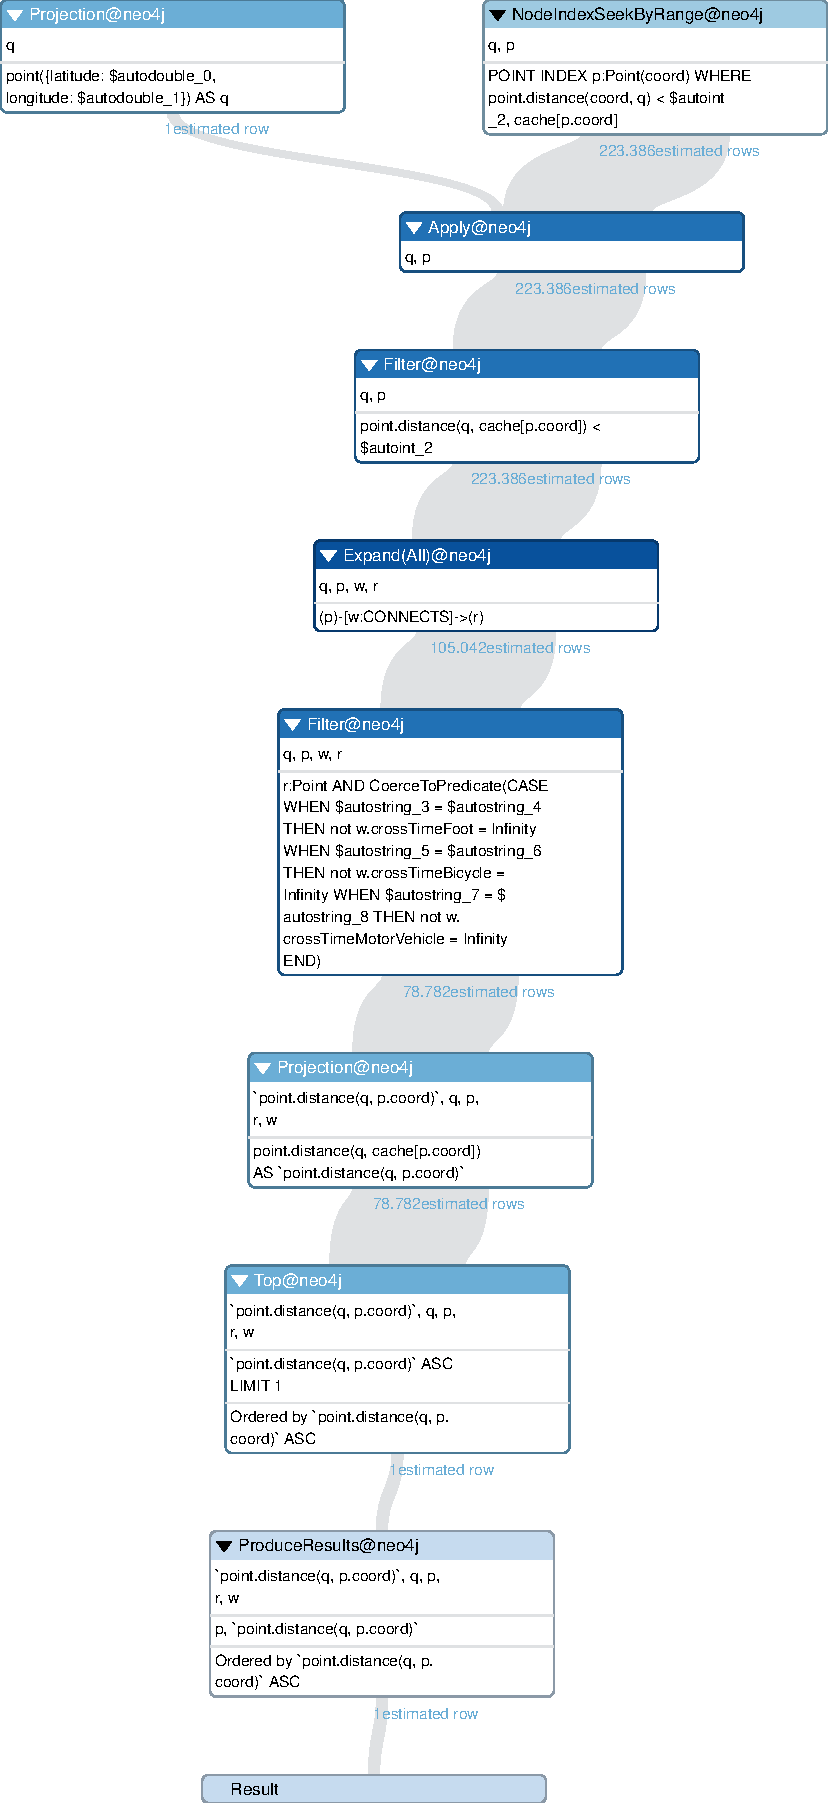
\includepdf[height=\textheight]{assets/plan_point_search_graph.pdf}

\paragraph{Benchmark}





